\chapter{Experiments and Results} % Main chapter title

\label{chapter:spencer_results} % Change X to a consecutive number; for referencing this chapter elsewhere, use \ref{ChapterX}

\lhead{Chapter 11. \emph{Experiments and Results}} % Change X to a consecutive number; this is for the header on each page - perhaps a shortened title



\section{Laboratory Experiments and Analysis}
\label{subsec:case_study-spencer-lab_experiments}

To have a first validation of our system, we performed experiments in a laboratory.

In this setting, we used Motion Capture to track users, and a navigation software based on \cite{sisbotTRO2007,kruse12crossing}. This software add proxemics based costs to static humans in the environment, continuously predicting and avoiding future collisions with moving persons, while  simultaneously keeping the robot as close as possible to the planned path.

\begin{figure}[ht!]
	\centering
	\includegraphics[scale=0.2]{img/case_study/spencer/robotGuiding.png}
	\caption[Robot Guide laboratory experiment]{This figure shows the SPENCER robot guiding a user in a laboratory}
	\label{fig:case_study-spencer-robotGuiding}
\end{figure}

We performed experiments with a single user following a robot on a predefined path. Data from these experiments are shown in table \ref{table:case-study-spencer-experiment_results} and in figure \ref{fig:case_study-spencer-exp_lab_result}. We start by showing speed adaptation tests:
\begin{itemize}
\item \textit{Adapting slow and fast}. In these two tests (figure \ref{fig:case_study-spencer-robotGuiding}) we used our system to guide respectively a user that would like to move at a slow pace, and a user that would like to move at a fast speed.
\item \textit{No adaptation}. In this experiments the robot will not adapt to the speed of the user, setting its own pace and stopping if it is too far.
\end{itemize}

Looking at the data we can see that our system shows lower values for the variance of speed and distance, which means that after a certain time it is able to find a condition of equilibrium with the human follower. The \textit{no adaptation} system shows a significantly higher variance for both values, since the robot stopped several times to wait for a user. We will now show some tests regarding the proactive behaviors of the robot:

\begin{itemize}
\item \textit{Proactive slow and fast}. During the task, the robot proactively chooses to change pace, in the first case by slowing down and in the second by accelerating. In our tests the user adapted after some seconds to the robot's pace, but this behaviors should be studied in-depth in user studies.
\item \textit{Suspend with screen and with no reason}. In these tests we asked a user to stop during the task. In the first case the user stopped near an information screen. After detecting this event, the robot approached the user to offer information, which lead to the resumption of the task. In the second case the user stopped at a different point of the path. The robot was not able to detect the reason for the suspension of the task and so simply   issued a warning to the user, abandoning the task after some seconds.
\end{itemize}


\begin{table}
\caption[Experiment results on speed adaptation]{Experiment results: $d$ is the distance between the robot and the user, $s_r$ is the robot's speed, $s_h$ is the human's speed, $\mu$ is the average and $\Delta$ is the variation of the quantity. Distances are expressed in meters, velocities in meters for seconds.}
\centering
\begin{tabular}{ | c | c | c | c | c | }

\hline
  test name     & $\mu$ $distance$ & $\mu$ $speed$ $difference$ & $\Delta$ $distance$ & $\Delta$ $speed$ $difference$ \\
\hline
adapting slow & 2.82 & -0.03 & 0.64 & 0.02 \\
  \hline
  adapting fast & 1.38 & 0.00 & 0.29 & 0.01 \\
  \hline
  no adaptation & 3.08 & -0.09 & 1.04 & 0.07 \\
\hline
proactive slow & 1.45 & -0.06 & 0.04 & 0.10 \\
\hline
proactive fast & 2.66 & -0.11 & 0.63 & 0.01 \\
\hline
\end{tabular}
\label{table:case-study-spencer-experiment_results}
\end{table}

\begin{figure}[ht!]
	\centering
	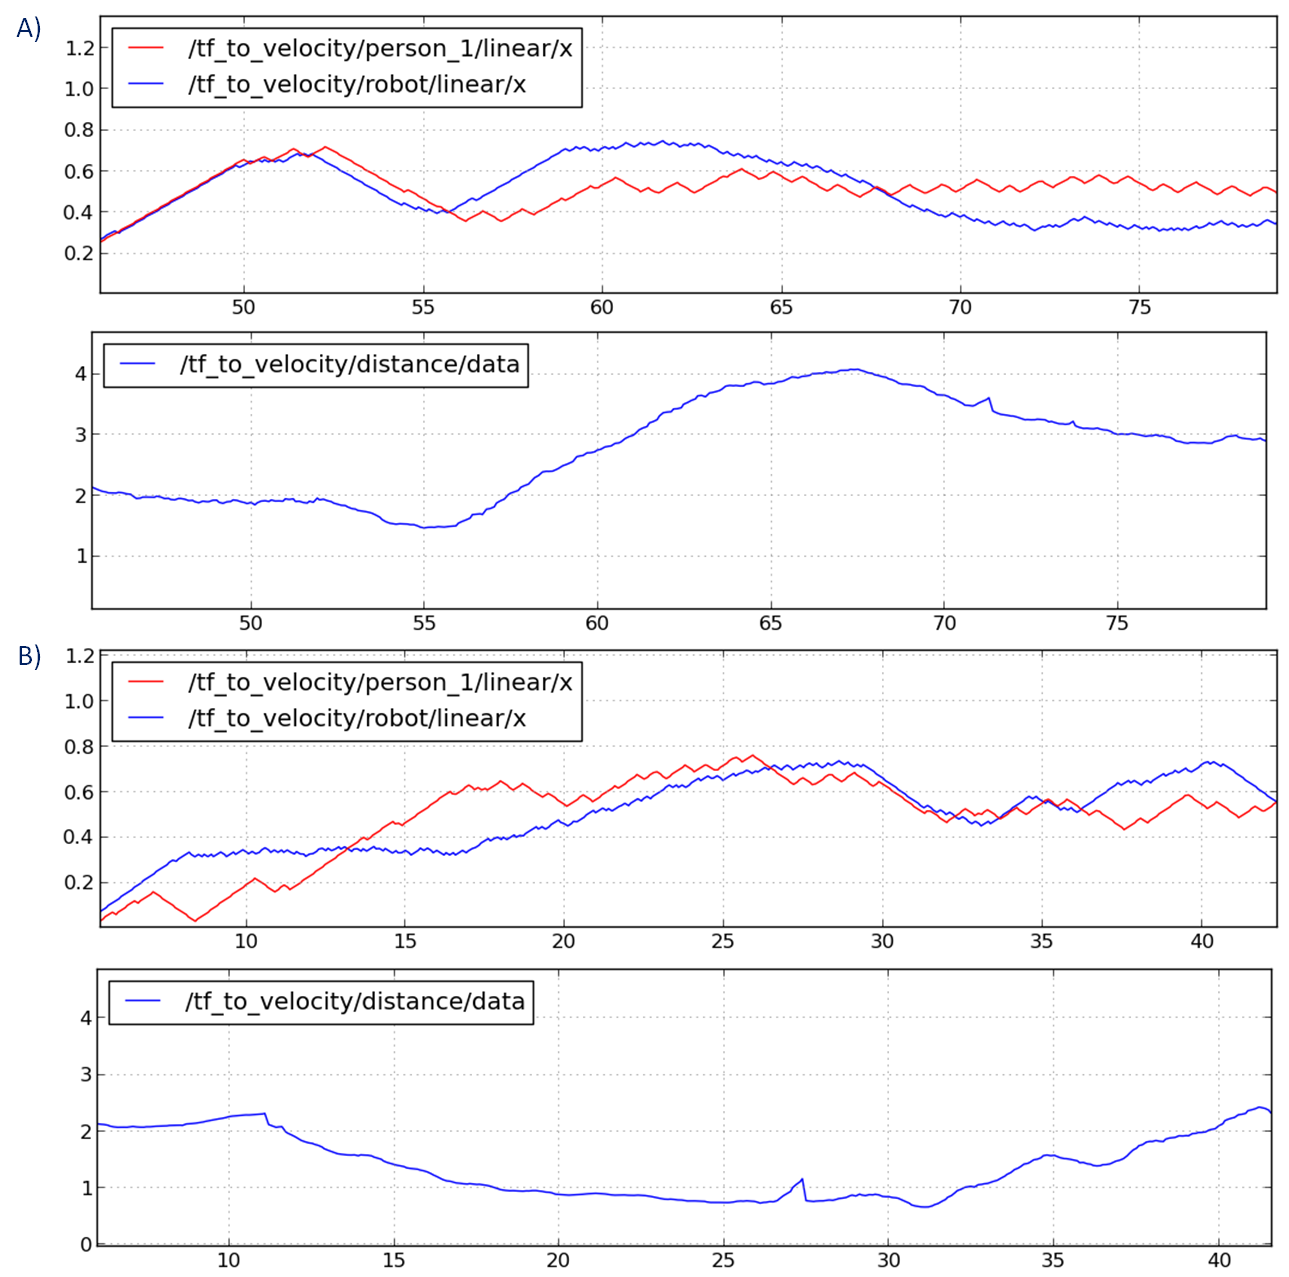
\includegraphics[scale=0.5]{img/case_study/spencer/experiments.png}
	\caption[Robot Guide laboratory experiment]{Robot Guide Laboratory Experiments: a) Adapting robot speed to a slow user. The first figure shows the speed of the user ($tf\_to\_velocity/person\_1/linear/x$) and of the robot ($tf\_to\_velocity/robot/linear/x$), and the second their distance. The robot starts slowing down at $t=60$, when the distance from the user is growing, until it finds an equilibrium with the user's speed. Notice that there is a turn in the path, at $T=50$, that causes the robot and the user to slow down. Distances are expressed in meters, velocities in meters for seconds.
b) Adapting robot speed to a fast user. As before, the figures show the robot and user's speed and their distance. The robot starts accelerating at $t=15$  when the distance from the user becomes small.}
	\label{fig:case_study-spencer-exp_lab_result}
\end{figure}

\section{Results on Airport Deployment}
\label{subsec:case_study-spencer-airport}
\subsubsection{Integration with Other Components}
The system was deployed in the Schiphol Airport for two different sessions, respectively of a week and of two weeks. In those weeks the team of the SPENCER project adapted the robot to the complex environment of the airport. Our system was integrated with several softwares from our partners, such as a combined laser-RGB people tracker, developed in \cite{lindermulti}, a novel localization approach, shown in \cite{kucner2015ndt}, a RTT based motion planner, shown in \cite{palmierirrt}, and cost-based social rules, introduced in \cite{okallearning}. More details on the whole SPENCER system are available in \cite{triebel2015spencer}.


\begin{figure}[ht!]
	\centering
	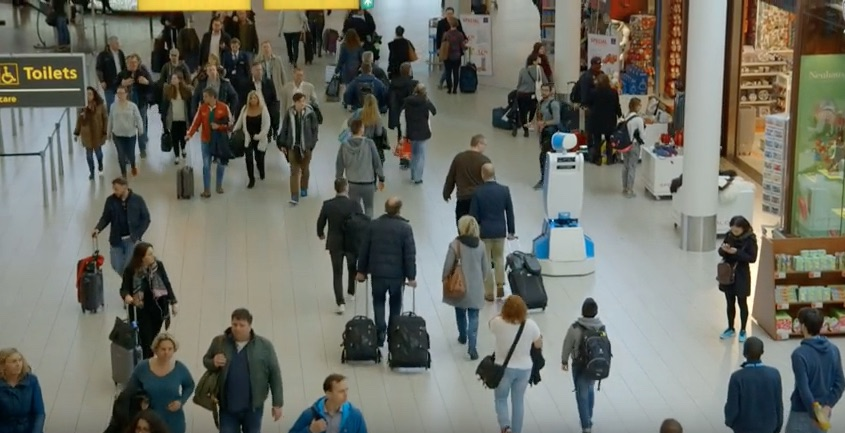
\includegraphics[scale=0.45]{img/case_study/spencer/spencer_schiphol.png}
	\caption{The robot moving in the Schipol airport}
	\label{fig:case_study-spencer-spencer_moving}
\end{figure}


\begin{figure}[ht!]
	\centering
	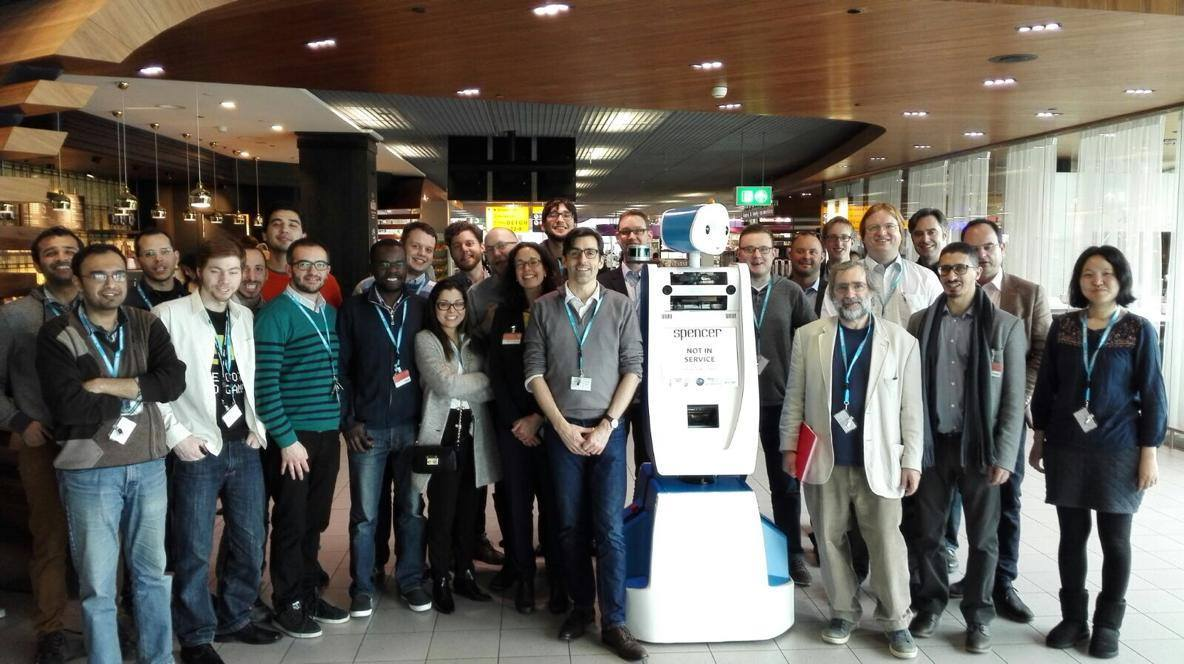
\includegraphics[scale=0.45]{img/case_study/spencer/all.jpg}
	\caption{The team that worked on the SPENCER project.}
	\label{fig:case_study-spencer-team}
\end{figure}

\subsection{User Study}

The system was tested in a user study, performed by researchers of the University of Twente\footnote{https://www.utwente.nl/en/}, which participated in the project. The study was conducted in two different days, with 18 participants, 11 males and 7 females, aged between 26 and 54. Ten participants indicated that the purpose of their journey was business, while eight indicated pleasure. Two different tests were performed:

\begin{itemize} 
\item In the first test the robot would pick up users at a chosen point, in Lounge-1 or in the Starbucks coffee shop of the airport, and guide them to a prefixed gate, B18. Users interacted with the robot by scanning special boarding passes created for this test on the robot's board pass reader, which prompted the start of the mission. To reach the gate, the robot had to pass through a crowded area, composed by several shops and other flight gates.
\item In the second test the robot met users at the gate B18 and guided them to Lounge-1. In this situation users initiated the mission by using the touchscreen display of the robot to select the destination.
\end{itemize}

At the end of each test, we collected three different kind of measures:
\begin{enumerate}
\item An individual feedback questionnaire where the users evaluated several aspects of the robot, like its behavior and aspect, on a 7-point Likert scale. In the day of testing two new questions where introduced about the robot, and a question on the participant's opinion on the robot in general.
\item A group interview, where users could discuss about their first impression of the robot, their experience in the test, and their thoughts on how to improve the systemm.
\item  Notes taken by researchers during guide, that helped to contextualize the results of users and to record specific events that occurred during tests.
\end{enumerate}


\begin{figure}[tb]
  \begin{center}
  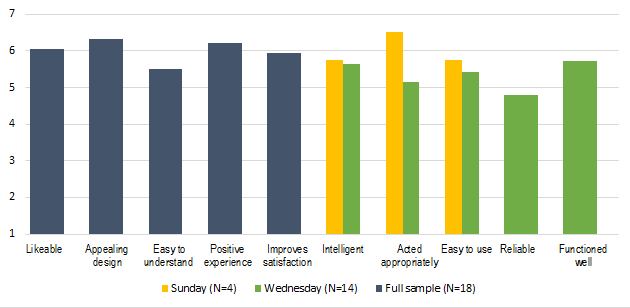
\includegraphics[width=0.95\textwidth]{img/case_study/spencer/graph_subjective_questions.png}
  \end{center}
  \caption{Answers to feedback questionnaire}
  \label{fig:feedback_questionnaire}
\end{figure}


Figure~\ref{fig:feedback_questionnaire} shows the results of the feedback questionnaire. Two questions were reformulated between the two days of testing, and so we included means for both of them. While the number of tests conducted were too limited to generalize, we can affirm that the participants had in general a positive impression of the robot. We list the main results of this test.

\begin{itemize}
\item Participants were generally happy with the robot's guiding performance.
\item The robot can be described as friendly-looking, easy-to-use and reliable.
\item The main issues encountered by users where related to the boarding card reader of the robot, and to its frequent abrupt stoppings.
\item Some users considered the speed of the robot too fast, or too slow, for their experience.
\item Users thought that the robot guide could be useful for people inexperience with flying, or new to a particular airport.
\item Users thought that the robot improved their customer satisfaction.
\item The main improvements for the robot include technical improvements, in particular related to the frequent stopping, and the addition of new functionalities, like carrying luggage or guiding to shops and restrooms.
\end{itemize}

\subsection{Discussion}
The experience in the airport showed the complexity of deploying a robot in such a complex scenario, interacting with inexperienced users. From our experiments we noticed several things:
\begin{itemize}
\item It is important to not make too many assumption about how users will interact with the robot. We expected users to follow the robot, staying mostly on its rear or side regions. This was not always true. In fact, several users were more interested in moving ahead of the robot, often concentrating on its behaviors more than on following it. The robot should adapt to these behaviors and not consider them as errors.
\item Human-Aware motion in complex environments is still a hard problem. Adapting the robot's speed was not simple, because the robot had stop or slow down often to avoid obstacles. Some times false positives generated by perception can lead to abrupt stops by the robot, which are seen as annoying and unnatural by users, and could even be dangerous.
\item Users are fascinated by robots, and are willing to ignore errors generated by the systems in short-term experiences.
\item It is important to perform long deployments in similar scenarios with real users. A long time in the three weeks where we worked at the airport was spent adapting the robot to the scenario. Longer deployments would allow for an iterative process of design-implementation-study.
\end{itemize}
